\documentclass{article}


\usepackage{arxiv}

\usepackage[utf8]{inputenc} % allow utf-8 input
\usepackage[T1]{fontenc}    % use 8-bit T1 fonts
\usepackage{hyperref}       % hyperlinks
\usepackage{url}            % simple URL typesetting
\usepackage{booktabs}       % professional-quality tables
\usepackage{amsfonts}       % blackboard math symbols
\usepackage{nicefrac}       % compact symbols for 1/2, etc.
\usepackage{microtype}      % microtypography
\usepackage{lipsum}
\usepackage{graphicx}
\usepackage{subcaption}
\usepackage{bbm}
\usepackage[toc,page]{appendix}
\usepackage{float}
\usepackage{mathtools}

\title{A survey on Attention Based Deep Learning Models in Natural Language Processing}

\author{
  Aryan Sharma\\
%  \thanks{Thanks to Prof. Boris Hanin.} \\
  Department of Computer Science\\
  Texas A\&M University\\
  College Station, TX \\
  \texttt{aryans@tamu.edu}
}

\begin{document}

\maketitle

\begin{abstract}

	Deep learning has employed multiple processing layers to learn hierarchical representations of data, and have produced state-of-the-art results in many domains including Natural Language Processing. In this report, we provide a survey on popular methods to represent language and text and review significant sequence to sequence deep learning models that have been disruptive for numerous NLP tasks, specially in the area of Neural Machine Translation. We specifically surveyed the development of attention in recurrent neural networks that have been phenomenal in extracting more context from the natural language and have paved way for some of the successful production ready Neural Machine Translators.

\end{abstract}


\section{Introduction}

	Natural Language Processing is a field that covers computer understanding and manipulation of human language. Today in the era of powerful search engines, where millions of webpages can be processed in less than a second, and diverse AI chatbots, NLP has enabled computers to perform a wide range of natural language related tasks at all levels, ranging from parsing and part-of-speech (POS) tagging, to machine translation and dialogue systems.
	
	Recently, Deep Learning architectures and algorithms have proved to be effective in the area of Computer Vision and Pattern Recognition. Following this, recent NLP research have evolved from context based statistical distributions to deep layered neural architectures, which has proved to be disruptive even in its rudimentary stages. Earlier most of the machine learning approaches were centered around shallow models like SVM, Logistic Regression etc. They were trained on very high dimensional and sparse features \cite{salton} which depends heavily on time-consuming and often incomplete hand-crafted features. 
	
	This research trend was however changed with the introduction of word embeddings and deep learning methods which enabled multi-level automatic feature representation learning. This survey explores the trends in few of those special models like LSTM, GRU, and specifically Attention models applied in the area of Machine Translation and Text Understanding. We present a timeline of models that have used and developed attention in the sequence to sequence recurrent neural networks and how it had evolved. Finally we present Google's GNMT which is the state of the art machine translator based on LSTMs, attention and residual networks. 
	

\section{Data representation using Word Embeddings}
\label{sec:emb}

	Like in many other fields, the representation of data and the method in which it is encoded and shown to machine learning algorithms, is often an important and fundamental part of a Machine Learning task. The effectiveness and scalability of the representation largely determine for the performance of the downstream machine learning model and application. Traditional representations treated words as atomic units and vector spaces\cite{salton} and most of the analysis was carried out on the basis of statistical distribution\cite{jones}, like word frequency, tf-idf \cite{jonesfre} etc. These choices, however simple and robust they may seem, are at limits in many tasks. The performance is usually dominated by the sheer size of the data.
	
	These led to the development of distributed representations of words existing in low-dimensional space called word embeddings, which captured context similarity and due to its smaller dimensionality, are fast and efficient in computing core NLP tasks. In 2003, Bengio et al. \cite{benn} proposed a neural network language model by learning a distributed representation for words which allows each training sentence to inform the model about an exponential number of semantically neighboring sentences. However word embeddings became popular when Mikolov et. al. introduced the Skip-gram model \cite{mikw2v} which is an efficient method for learning high quality vector representations of words from large amounts of unstructured text data. Below in \ref{sec:w2v} we discuss the salient features of that paper. In the section \ref{sec:embdim} we surveyed evaluation of how using different types of context to learn word embeddings affects performance on a wide range of intrinsic and extrinsic NLP tasks \cite{melamud}.
	
\subsection{Word2Vec}
\label{sec:w2v}
	
	Mikolov et al. \cite{mikw2v} \cite{mikngs} proposed CBOW and Skip-Gram models in 2013. The CBOW model calculates the conditional probability of a target word given the context words surrounding the the target word across a window of size \(k\). Skip-Gram model, on the other hand, predicts the probabilities of potential surrounding context words given the central target word. The context words are assumed to be located symmetrically around the target words within a window in both directions. The accuracy of the prediction, as shown in the paper, increases as we increase the embedding dimension. This is essentially giving more context, and thus more accuracy, to the model. The accuracy converges at a certain dimnesion, where we get the optimal embedding dimension. 
	
	Both the models are a fully connected Neural Network with one hidden layer as shown in Figure \ref{fig:w2v}. In the CBOW model, the input layer takes one-hot encoding of context word that has \(V\) neurons, which is in turn fully connected to the hidden layer which has \(N\) neurons by a weight matrix \(W \in \Re^{V \times N}\). The output layer in the basic word2vec is the softmax of all the word in the vocabulary which is connected to the hidden layer using a weight matrix \(W' \in \Re^{H \times V}\). Each word (say \(k^{th}\)) in the vocabulary is then represented by two vectors \(u_c = W_{(k,...)}\) and \(v_t = W'_{(...,k)}\). The Skip-Gram model is the exact opposite of this model where the output are multiple context vectors and the input is a context word vector. The cost funtion to optimize is \(log( p(w_{o} | w_i))\) where,
	\[p(w_{o} | w_i) = \frac{e^{u_0^Tv_c}}{\sum_{w=1}^{W} e^{u_w^Tv_c}}\]
	
	There were however limitations to these models. They were unable to represent phrases where the combination of meanings of individual words did not represent the collective meanings. Another problem was with the huge size of the neural network which made the model computationally expensive. These problems were explored in \cite{mikngs} by Mikolov et al. They proposed the idea of identifying phrases on the basis of word co-occurence and training the embeddings for them separately. However, the main idea of this paper was about making it more effecient computationally. They proposed the idea of subsampling where there was a probability associated with common occuring words like 'the', which didn't provided much information about the context. Based on this probability they decided to drop or keep the word for training. Another method proposed was that of 'Negative Sampling' which replaced the hierarchical
	softmax method. It addressed the issue of sparsity of updates happening to the weight matrices. Negative sampling selects small number of negative words (words for which we want the output of 0) and update the weight for this small set along with the postitive word (which is the most probable answer that we want). The final cost function of the model is then: 
	\[J(\theta) = \sum_{PAIRS} [log(\sigma(u_{W_O}^Tv_{W_I}) + \sum_{i=1}^{k} \mathbb{E}_{w_i \sim P_n(w)} [log(\sigma(u_{W_i}^Tv_{W_I})])] \] 

	\begin{figure}
		\centering
		\begin{subfigure}{0.4\textwidth}
			\centering
			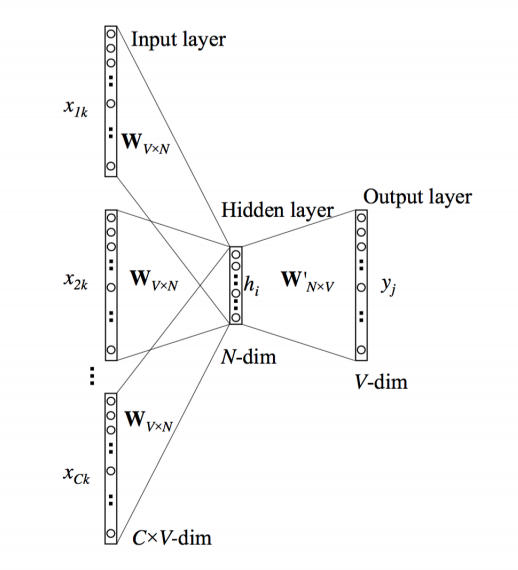
\includegraphics[width=1\textwidth]{fig/cbow.png}
			\caption{CBOW model which predicts the target word from multiple one-hot encoding of context word vectors}
		\end{subfigure}
		\hspace*{2em} % separation between the subfigures
		\begin{subfigure}{0.4\textwidth}
			\centering
			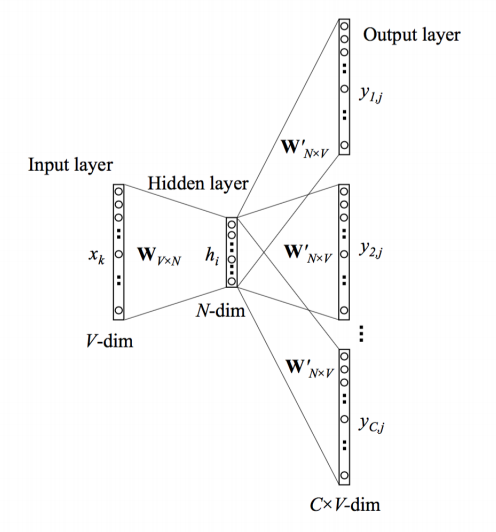
\includegraphics[width=1\textwidth]{fig/skipgram.png}
			\caption{Skip-Gram model which on the other hand predicts the context vectors of a given a target word}
		\end{subfigure}
		\caption{Word2Vec consists of two models as shown above. Every word has representation from both the embeddings}
		\label{fig:w2v}
	\end{figure}

\subsection{Role of Context Types and Dimentionality in Learning Word Embeddings}
\label{sec:embdim}

	Word embeddings are evaluated on \textit{intrinsic} and \textit{extrinsic} tasks. Intrinsic tasks mostly include predicting human judgments of semantic relations between words whereas extrinsic tasks include various 'real' downstream NLP tasks, such as coreference resolution and sentiment analysis. Recent works have shown that while intrinsic evaluations are easier to perform, their correlation with results on extrinsic evaluations is not very reliable. In the work by Melamud et al. \cite{melamud}, an extensive evaluation of word embeddings learned with different types of context has been provided. It compared window based embeddings with dependency-based word embeddings and substitute based word embeddings. The task was performed for Dependency Parsing, Named-Entity-Recognition, Coreference Resolution, and Sentiment Analysis. 
	
	They observed that while the performance improved as the number of dimension increases, there was significant difference using different types of context. It was more evident in WordSim-353-R task which includes 353 word pairs manually annotated with a degree of similarity and focuses on functional and topical similarities. The performance decreased with decrease in window size and the largest window embedding performed the best. For the extrinsic tasks, they observed that performance degraded with using too man dimensions. This was in contrast to intrinsic task where higher dimentionality usually yields better results. They also combined the embeddings by simple concatenation and found that the performance depended on the dimensionality and the task at hand. 

\section{Advancement of Recurrent Neural Networks in NLP}
\label{sec:seqnlp}

	Deep Neural Networks (DNN) have been successful in many difficult learning tasks. Despite their flexibility and power, they cannot be used to map sequences to sequences and are only valid for problems whose inputs and targets can be sensibly encoded with vectors of fixed dimentionality. This is a huge limitation since most problems can be best expressed with sequences whose lenghts are not know a-priori. This lead to the idea of Recurrent Neural Networks (RNNs).
	
	RNNs has the ability to capture the inherent sequential nature present in the language and is tailor made for modeling context dependencies in NLP. They are also effective in encoding a variable length of text, including long sentences, paragraphs and even documents (Discussed in Appendix \ref{sec:rnn}). Unlike CNN, RNN have flexible computational steps that provide better modeling capability and create possibility to capture unbounded context. The basic RNNs suffered from the problem of vanishing gradient (Discussed in Appendix \ref{sec:van}) and thus led to the development of Gated Recurrent Networks(GRU) (Discussed in Appendix \ref{sec:gru}), Long Short Term Memory(LSTM) (Discussed in Appendix \ref{sec:lstm}).
	
	In this section, we surveyed the papers that have used the variants of RNNs in NLP. In Sutskevar et al. \cite{suts}, a general end to end multi layered sequence learning model was proposed. This pioneering model in LSTM is discussed in \ref{sec:suts}. In \ref{sec:pos} we discuss a deep Bi-LSTM model from Plank et al. \cite{pos}, which combines the POS tagging loss function with an auxiliary loss function that accounts for rare words. There has been a lot of reserach in the area of opinion mining and sentimet analysis about reviews of products. We discuss a paper from Ruder et al. in \ref{sec:senti}, in which a hierarchical bidirectional LSTM is proposed and is shown to out-perform non-hierarchical models. It builds upon the intuition that sentences in a review elaborate and build upon each other. All these section focuses on the develpment of RNN (or LSTM and their variants) as a plausible model to construct state of the art NLP tools. 

\subsection{Sequence to Sequence Learning with Neural Networks}
\label{sec:suts}
	
	In the paper \cite{suts}, the authors applied multi-layered Long Short-Term Memory (LSTM) (Appendix \ref{sec:lstm}) to map input sequence to a vector of fixed dimentionality. Given a sequence of inputs \((x_1, ... , x_T)\), a standard RNN computes a sequence of outputs \(y_1, ..., y_T\) by iterating the following equations:
	\[h_t = sigm(W^{hx} x_t + W^{hh} h_{t-1})\]
	\[y_t = W^{yh} h_t\]
	
	As is evident, RNNs can map sequences to sequences whenever the alignment between the inputs and the outputs is known. However, it becomes difficult when input and output sequences have different lengths with complex non-monotonic relationship. A simple strategy of encoding the input in a fixed sized vector can lead to long term dependencies and can be difficult to train. Therefore the authors decided to use LSTMs which has shown to perform better in learning long term dependencies. This paper was one of the rudimentary papers in exploring the power of LSTMs in Neural Machine Translation and sequence processing, upon which many state-of-the-art encoder-decoder models were developed. 
	
	\paragraph{Encoding:} LSTMs estimate the conditional probability \(p(y_1, ..., y_{T'} | x_1, ..., x_T)\) where \((x_1, ..., x_T)\) is an input sequence and \((y_1, ..., y_T')\) is the corresponding output sequence whose length \(T'\) can differ from \(T\). The decoder LSTM uses the fixed dimentional representation \(v\) of the input sequence, given by the last hidden state of the encoder LSTM. The last hidden state was determined when the input sequence received special <EOS> token which marked the end of the sequence. The probability of \(y_1, ..., y_{T'}\) is computed as below and each distribution as represented as softmax over all the words in the vocabulary:
	\[p(y_1, ..., y_{T'} | x_1, ..., x_T) = \prod_{t=1}^{T'} p(y_{T} | v, y_1, ..., y_{t-1})\]
	
	\paragraph{Decoding:} The training involved the maximization of log probabilities of a correct translation \(T\) given a source sentence \(S\). The training objective is:
	\[1/|\Psi| \sum_{(T,S) \in \Psi} log(p(T|S)\]
	
	where \(\Psi\) is the training set. After training the most likely translation is produced using a simple left to right beam decoder which maintains a small number \(B\) of partial hypotheses (prefix of some translation). At every timestep, these hypotheses are extended with every possible word and \(B\) most likely hypotheses are kept according to the model's log probability. 
	
	\paragraph{Difference from standard encoder-decoder models: }The model in this paper differs with the standard encoder-decoder model in three ways. First, by using two LSTM (output and input), they utilized the increased number of parameters to train the LSTM of multiple language simultaneously. Second, they stacked four layers of LSTM which they found to significantly out-perform shallow LSTMs. Also one of the most significant trick introduced in this paper was to reverse the input sequence (and not the output sequence), before feeding it into the network. The author's believed that it is caused by the introduction of any short-term dependencies to the dataset, where in the normal case each word in the source sentence is far from its corresponding word in the target sentence.
	
\subsection{Multilingual Part-of-Speech Tagging with Bidirectional Long-Short-Term-Memory models with Auxiliary Loss}
\label{sec:pos}

	LSTMs are recurrent neural networks in which layers are deigned to prevent vanishing gradients. Bidirectional LSTMs make a forward and backward pass thorugh the sequence before passing on to the next layer. This paper evaluated this model across 22 languages and compared performance with representation at different levels of granularity (words, characters, and bytes). 
	
	A biRNN reads the input twice from both directions, and their encodings are concatenated. There are two flavors of biRNN: sequence biRNN (\(biRNN_{seq}\)) and context biRNN (\(biRNN_{ctx}\)). In the former, the input is a sequence of vectors \(x_{1:n}\) and the output is the concatanation \((\circ)\) of a forward \((f)\) and reverse \((r)\) RNN each reading the sequence from a different direction. In the context biRNN, there is an additional input \(i\), which indicated the sequence position. The resulting vector \(v_i\) is a concatanation of RNN encodings upto \(i\). 
	
	\[v = biRNN_{seq} (x_{1:n}) = RNN_f(x_{1:n}) \circ RNN_r(x_{n:1})\]
	\[v_i = biRNN_{ctx} (x_{1:n}, i) = RNN_f(x_{1:i}) \circ RNN_r(x_{n:i})\]
	
	As shown in Figure \ref{fig:pos}, this paper proposed a context bi-LSTM tagging model taking the input as word embedding \(\overrightarrow{w}\). After computing the subtoken level (character \(\overrightarrow{c}\) or unicode byte \(\overrightarrow{b}\)) embeddings of words using a sequence Elation HealthLSTM at the lower level, it is then concatenated with the (learned) word embeddings vector \(\overrightarrow{w}\) which forms the input to the context Elation HealthLSTM at the next layer. 
	
	In addition to the POS tagging, this paper also trains the Elation HealthLSTM tagger to predict a label that represents the log frequency of the next token as estimated from the training data. This is shown in the left side of Figure \ref{fig:pos}. Besides using the combination of character embeddings \(\overrightarrow{c}\) and \(\overrightarrow{b}\), the authors also tested only using characters \(\overrightarrow{c}\) and found it to perform well. 
	
	\begin{figure}
		\centering
		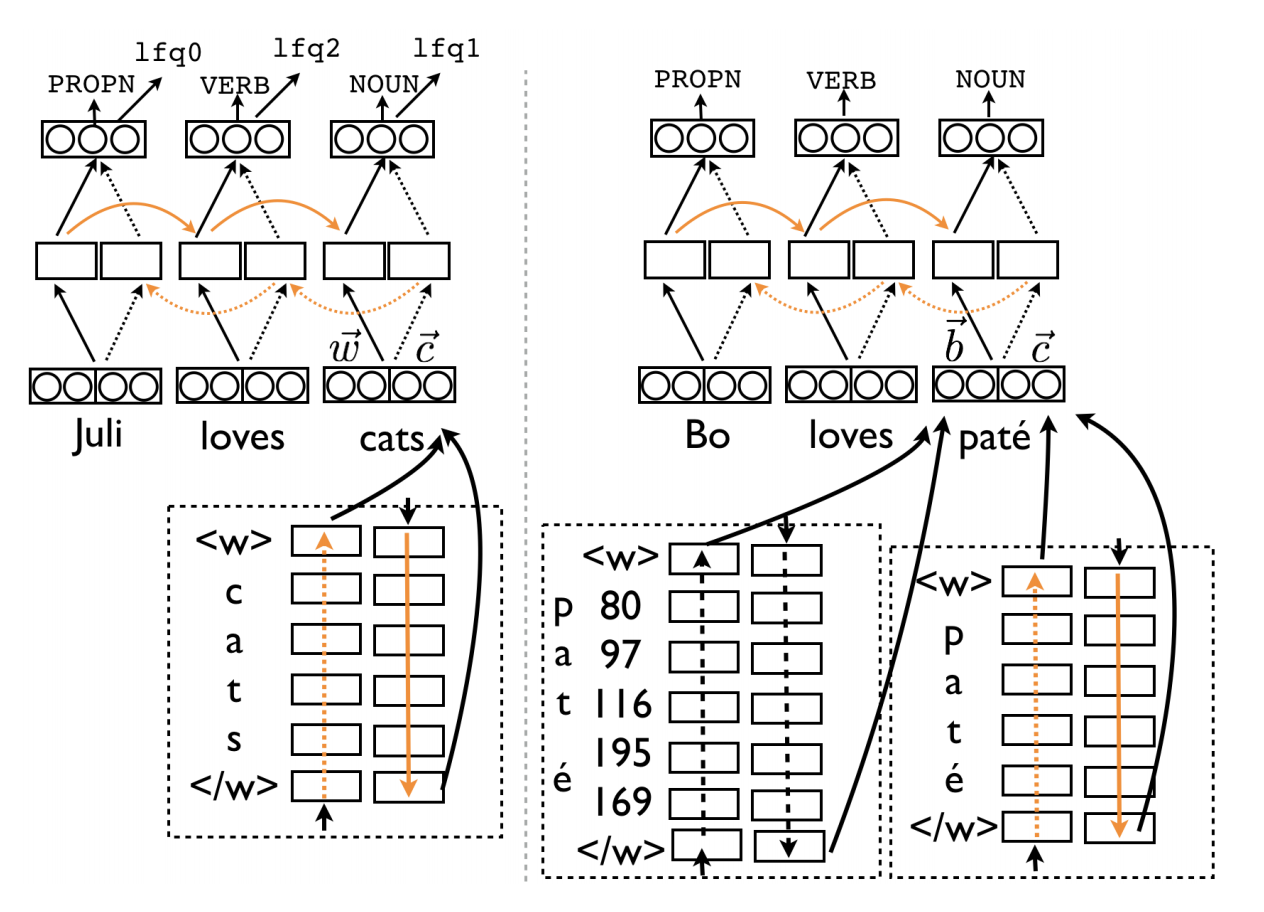
\includegraphics[width=0.6\textwidth]{fig/pos.png}
		\caption{\textit{Left}: Multi-task Elation HealthLSTM that predicts the tag and frequency class for the next token at every time step. \textit{Right}: Elation HealthLSTM using characters embeddings + byte embeddings}
		\label{fig:pos}
	\end{figure}

\subsection{Aspect-Based Sentiment Analysis}
\label{sec:senti}

	This work from Ruder et al. \cite{senti} builds on the fact that knowledge about the relations and the sentiment of surrounding sentences inform the sentimet of the current sentence. The Neural Network based work on Sentiment analysis before this paper focused on intra-sentence relations such as \textit{Background} but failed to capture inter-sentence relations like \textit{Elaboration} that rely on discourse structure and provide valuable information for sentiment prediction. Also the previous works needed some or the other feature engineering, or positional information, or parse trees which are often unavailable for low-resource language. This paper requires none of that and showed better results than sentence-level CNN and sentence level Elation HealthLSTM baselines. 
	
	\paragraph{Input Preprocessing:} Before feeding into the network, the reviews' sentence representation requires some pre-processing. Each review is padded to a length \(l\) by inserting padding tokens. Each review, in turn, is padded to length \(h\) by inserting padding sentences. Each sentence is represented as a concatenation of its word embeddings \(x_{1:l}\) where \(x_t \in \Re^{k}\) is the \(k\)-dimensional vector of the \(t\)-th word in the sentence. Every sentence is associated with an aspect which consists of an entity and an attribute, eg. \texttt{SERVICE\#GENERAL}. Every aspect \(a\) is the average of its entity and attribute embeddings \(\frac{1}{2}(x_e+x_a)\) where \(x_e, x_a \in \Re^m\).
	
	\paragraph{Model:} There are two level of hierarchy of Elation HealthLSTM layers over the word embeddings and before the output layer. As shown in Figure \ref{fig:senti}, the sentence level forward and backward LSTMs receive the sentence starting with the first and last word embedding \(x_1\) and \(x_l\) respectively. The final output \(h_l\) of both LSTMs is then concatenated with the aspect vector \(a\) and is then fed as input into the review-level forward and backward LSTMs. The outputs of both the Elation HealthLSTMs are than concatenated and fed into a softmax layer, which provides a probability distribution over sentiments for each sentence. 
	
	\begin{figure}
		\centering
		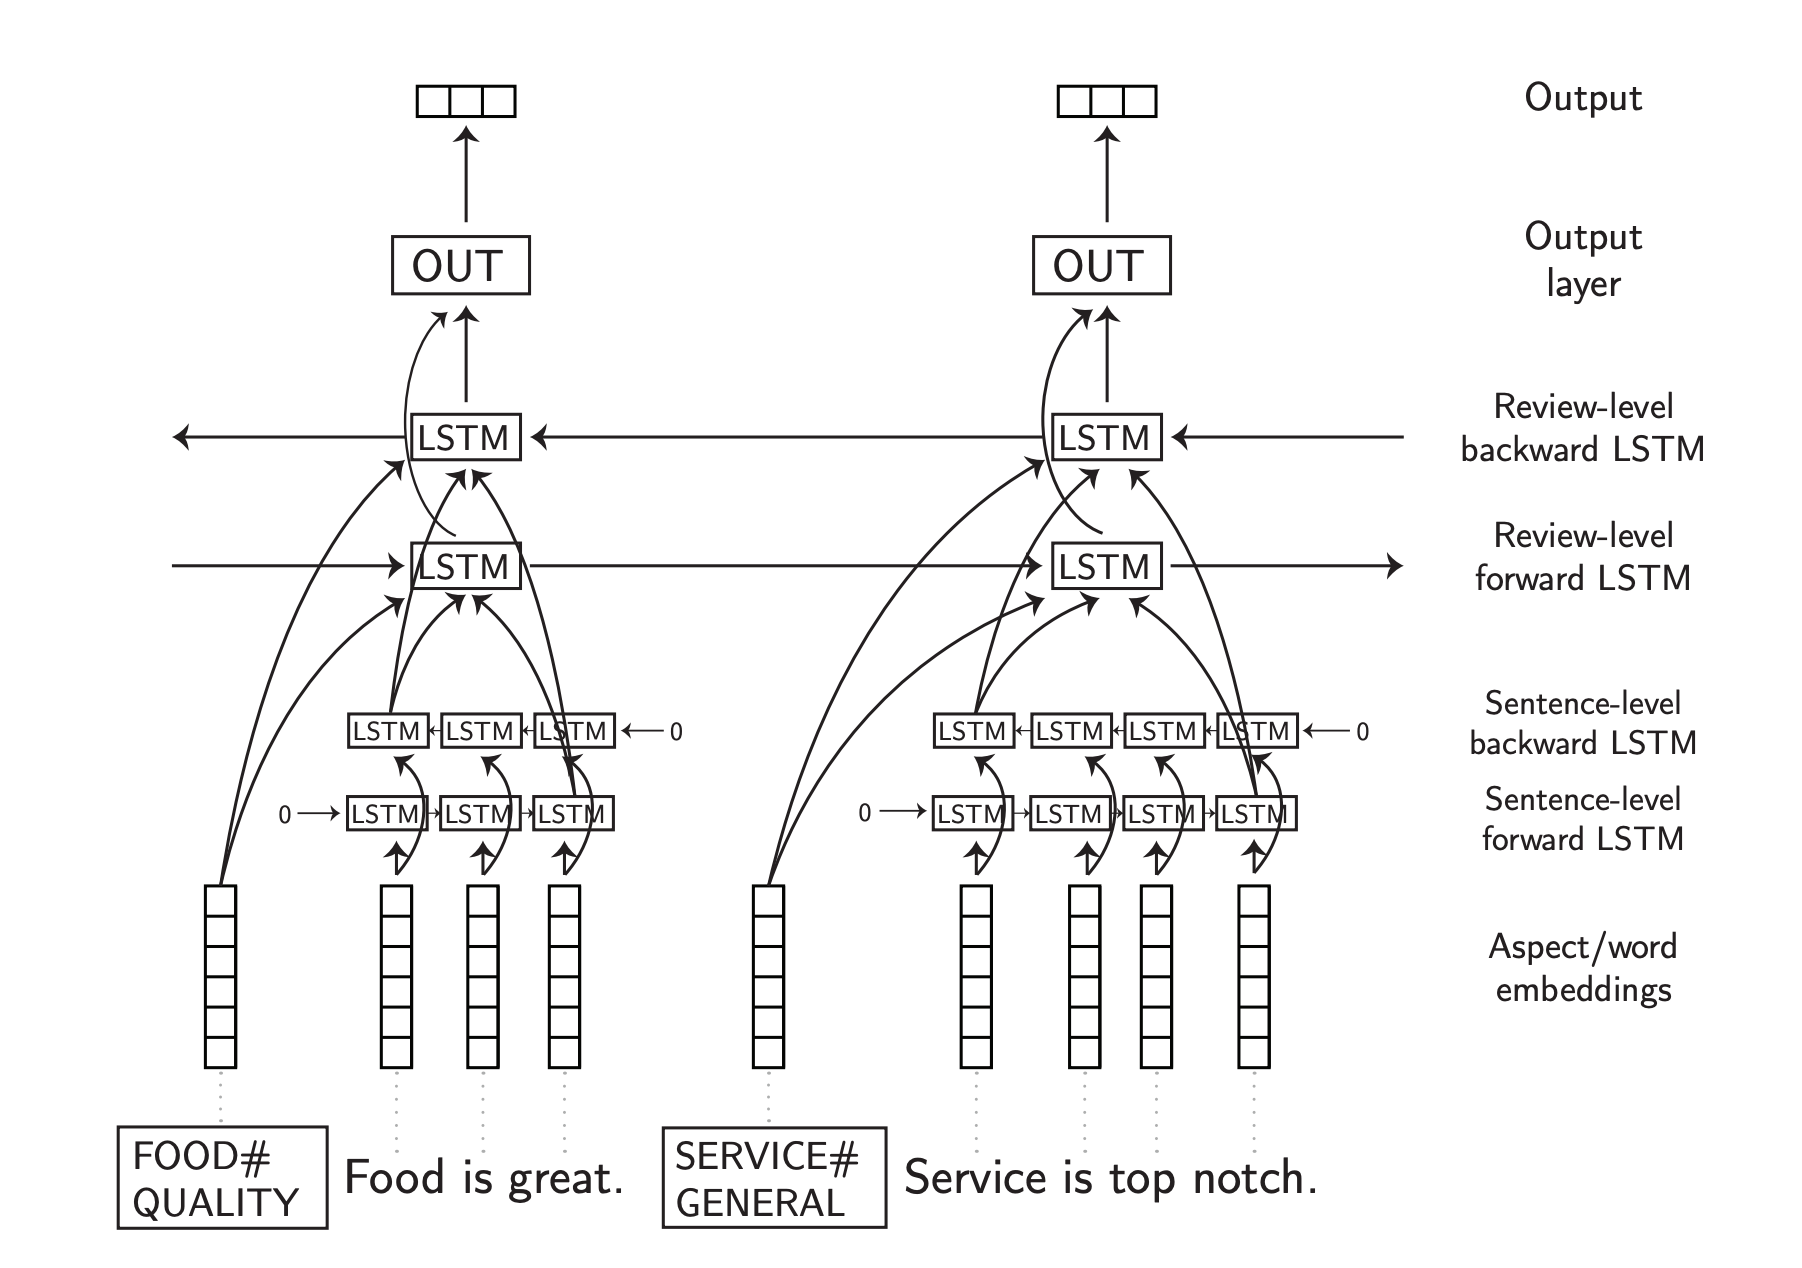
\includegraphics[width=0.6\textwidth]{fig/senti.png}
		\caption{The hierarchical Elation HealthLSTM model for aspect-based sentiment analysis}
		\label{fig:senti}
	\end{figure}

\section{Attention based Deep Learning Models for Natural Language Processing}
\label{sec:attention}

	One potential problem with the traditional encoder-decoder fraework has is that the encoder at times is forced to encode information which might not be fully relevant to the task at hand. Also this problem exacerbates when the input is long or very information rich and selective encoding is not possible. In tasks such as text summarization and machine translation, ther is certain alignment existing between the input text and the output text. Thus certain part of the input text is hihgly related to each token generation step. This intuition inspires the attention mechanism. Attention attempts to ease the above problems by allowing the decoder to refer back to the input sequence.
	
	In the following sections, we surveyed the development of attention in NLP, and specifically machine translation, text and sentiment analysis. In section \ref{sec:bahnmt}, we discuss the NMT based on alignment proposed in Bahdanau et al. \cite{bahattn}. We then moved to a simplified version of attention based NMT proposed by Luong et al. \cite{luongatn}. It talked about global and local aproaches and multiplicative attention that provides a much simpler computational path as compared to \ref{sec:bahnmt}. Attention cannot only be used to attend to encoder or previous hidden states, but also to obtain a distribution over other features, such as the word embeddings of a text as used for reading comprehension (Kadlec et al., \cite{kadlec}). Section \ref{sec:kadlec} talks about it. However, attention is not directly applicable to classification tasks that do not require additional information, such as sentiment analysis. In such models, the final hidden state of an LSTM or an aggregation function such as max pooling or averaging is often used to obtain a sentence representation. In section \ref{sec:lin}, we survey methods to extract word embedding usign self-attention. 

\subsection{Neural Machine Translation by jointly learning to align and translate}
\label{sec:bahnmt}

	Neural machine translation (NMT) aims at building a single neural network that can be jointly trained maximize the translation performance. As mentioned before, the traditional encoder-decoder model compresses all the necessary information of source sentence into a fixed-length vector and makes it difficult to deal with long sentences. The model proposed by Bahdanau et al. \cite{bahattn} addresses this issue by learning to align and translate jointly by encoding the input sentence into a sequence of vectors and choosing a subset of these vectors adaptively, unlike the traditional models. As we can see in Figure \ref{fig:bahatn}, the model correctly aligns itself with the reverse meaning of the French input shown. 
	
	\paragraph{RNN Encoder-Decoder: } The model proposed in this paper develops on the RNN Encoder-Decoder, proposed by Cho et al. \cite{cho}. In this framework, the encoder reads the input sentence, a sequence of vectors \(\textbf{x} = (x_1, ..., x_{t_x})\), into a vector \(c\). The following equations define the internal state of the RNN:
	\[h_t = f(x_t, h_{t-1})\]
	\[c = q({h_1, ..., h _{T_x}})\]
	where \(h_t \in \Re^n\) is a hidden state at time \(t\), and \(c\) is a vector generated from the sequence of hidden states. \(f\) and \(q\) are some non-linear functions. The decoder predicts the next word \(y_{t'}\) from the context vector \(c\) and all the previously predicted words \({y_1, ..., y_{t'-1}}\). Hence,
	\[p(\textbf{y}) = \prod_{t=1}^{T} p(y_t | y_1, ..., y_{t-1}, c)\]
	where \(\textbf{y} = (y_1, ..., y_{T_y})\). With an RNN, the conditional probability is modeled using \(g\), which is a non-linear multi-layered, function. 
	\[p(y_t | y_1, ..., y_{t-1}, c) = g(y_{t-1}, s_t, c)\]
	
	\begin{figure}
		\centering
		\begin{subfigure}{0.35\textwidth}
			\label{fig:bahatn1}
			\centering
			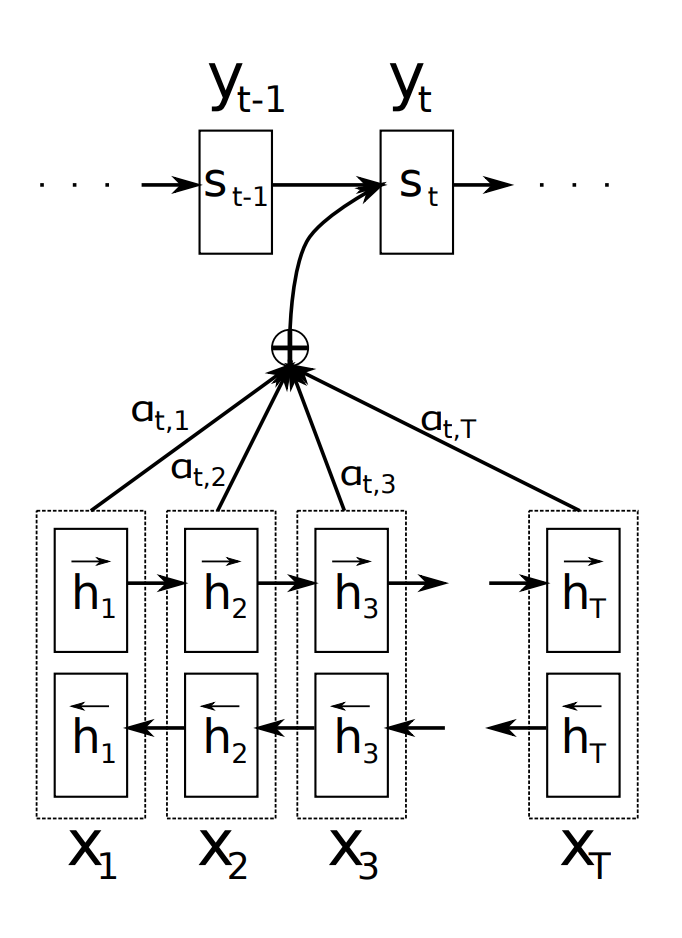
\includegraphics[width=1\textwidth]{fig/adatn1.png}
			\caption{The proposed model trying to generate the \(t^{th}\) target word \(y_t\) given a source sentence \((x_1,..., x_T)\)}
		\end{subfigure}
		\hspace*{2em} % separation between the subfigures
		\begin{subfigure}{0.45\textwidth}
			\label{fig:bahatn2}
			\centering
			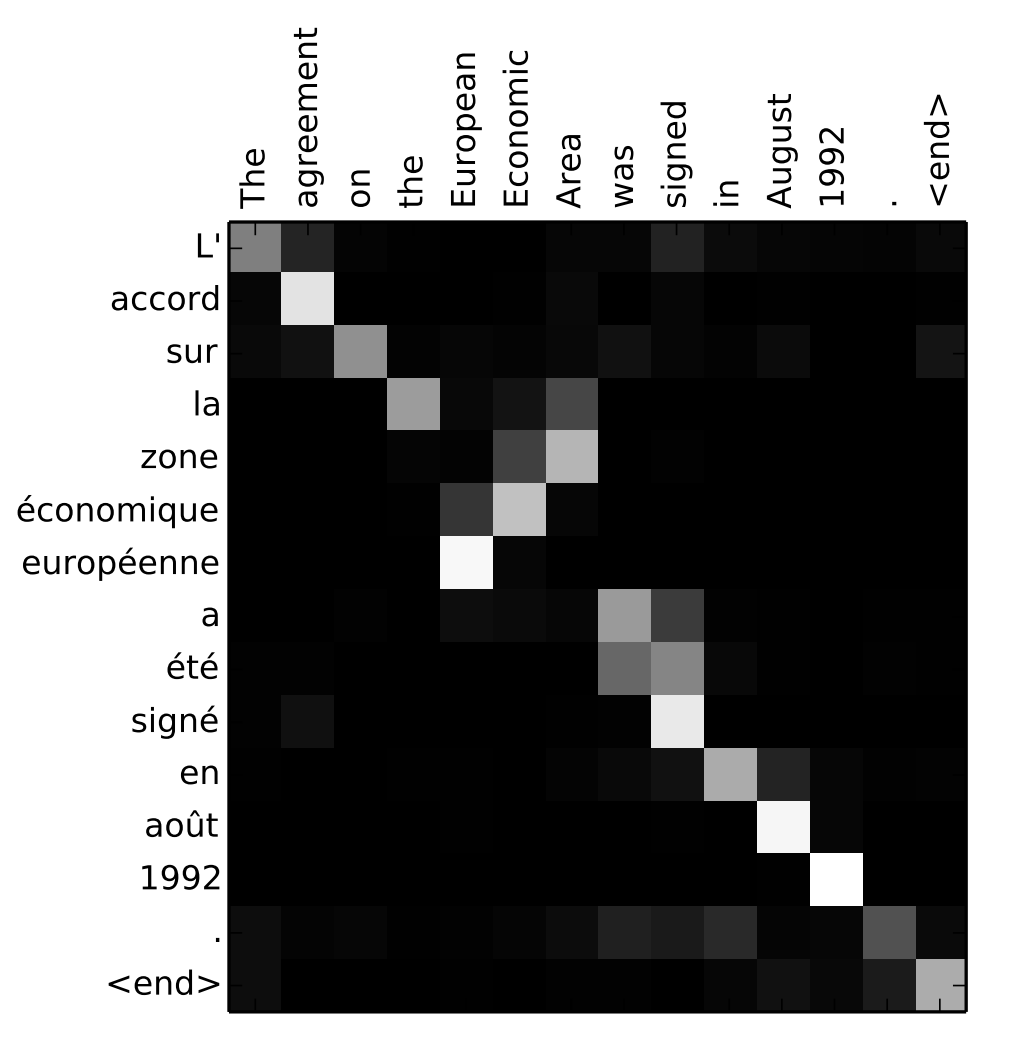
\includegraphics[width=1\textwidth]{fig/adatn2.png}
			\caption{Each pixel in this activation map shows the weight \(\alpha_{ij}\) of the annotation of the \(j^{th}\) source word for the \(i^{th}\) target word.}
		\end{subfigure}
		\caption{The model and the result from Neural Machine Translation by jointly learning to align and translate}
		\label{fig:bahatn}
	\end{figure}

	\paragraph{Encoder:} The authors decided to go with Elation HealthRNN as the encoder layer as they also wanted the annotation of each word to summarize the following words as well. We observe here that instead of the vanilla RNN, a new Gated Recurrent Unit has been used. It is a special version of LSTM and is described in detail in Appendix \ref{sec:gru}. The annotation for each word \(x_j\) is obtained by concatenating the forward hidden state \(\overrightarrow{h_j}\) and the backward \(\overleftarrow{h_j}\) ie. \(h_j = [\overrightarrow{h_j};\overleftarrow{h_j}]^T\).  
	
	The encoder takes input as a source sentence of 1-of-K coded word vectors \(\textbf{x}\) and outputs a translated sentence of 1-of-K coded word vectors \(\textbf{y}\)
	\[\textbf{x} = (x_1,..., x_{T_x}), x_i \in \Re^{K_x} \hspace{2em} \textbf{y} = (y_1,..., y_{T_y}), y_i \in \Re^{K_y}\]
	
	Here, \(K_x\) and \(K_y\) are the vocabulary sizes and \(T_x\) and \(T_y\) are the length of the source and target sentences. The forward states of the biRNN are computed as:
	\[\overrightarrow{h_i} = \mathbbm{1}_{i>0} [(1-\overrightarrow{z_i}) \circ \overrightarrow{h}_{i-1} + \overrightarrow{z_i} \circ \overrightarrow{\widetilde{h_i}}] \]
	where
	\[\overrightarrow{\widetilde{h_i}} = \tanh(\overrightarrow{W}E_{x_i} + \overrightarrow{U}[\overrightarrow{r_i} \circ \overrightarrow{h}_{i-1}])\] 
	\[\overrightarrow{z_i} = \sigma(\overrightarrow{W}_zE_{x_i} + \overrightarrow{U}_z\overrightarrow{h}_{i-1})\]
	\[\overrightarrow{r_i} = \sigma(\overrightarrow{W_r}E_{x_i} + \overrightarrow{U_r}\overrightarrow{h}_{i-1})\]
	
	\(E \in \Re^{m \times K_x}\) is the word embedding matrix. \(\overrightarrow{W}, \overrightarrow{W_z}, \overrightarrow{W_r} \in \Re^{n \times m}\), \(\overrightarrow{U}, \overrightarrow{U_z}, \overrightarrow{U_r} \in \Re^{n \times n}\) are weight matrices. \(m\) and \(n\) are embedding dimentionality and the number of hidden units respectively. Similarly the backward states \(\overleftarrow{h_i}\) are computed to get the whole annotations \(h_i\) for each word in the sentence. 
	
	The context vector \(c_i\) is then calculated as the weighted sum of these annotations \(h_i\):
	\[c_i = \sum_{j=1}^{T_x} \alpha_{ij}h_j \hspace{0.5em} where, \hspace{0.5em} \alpha_{ij} = \frac{exp(e_{ij})}{\sum_{k=1}^{T_x} exp(e_{ik})}\]
	\[e_{ij} = a(s_{i-1}, h_j) = v_a^T\tanh(W_as_{i-1} + U_ah_j)\]

	\(e_{ij}\) is an alignment model which shows how well the inputs around position \(i\) are aligned with inputs at position \(j\) and \(W_a \in \Re^n \times n, U_a \in \Re^{n \times 2n}\) and \(v_a \in \Re^n\) are the weight matrices. 
	
	\paragraph{Decoder: } Unlike the RNN model, the conditional probability here is conditioned on distinct context vector \(c_i\) for each target word \(y_i\). It is represented as:
	\[p(y_i | y_1, ..., y_{i-1}, \textbf{x}) = g(y_{i-1}, s_i, c_i)\hspace{1em} where \hspace{1em} 	s_i = f(s_{i-1}, y_{i-1}, c_i)\]
	The context vector \(c_i\) depends on a sequence of annotations \((h_1, ..., h_{T_x})\) to which an encoder maps the input sentence. Each annotation \(h_i\) contains information about the whole input sequence with a string focus on the parts surrounding the \(i^{th}\) word of the input sequence.
	
	The hidden state \(s_i\) of the decoder is computed by:
	\[s_i = (1-{z_i}) \circ {s}_{i-1} + {z_i} \circ {\widetilde{s_i}}\]
	where
	\[\widetilde{s_i} = \tanh(WE_{y_{i-1}} + U[{r_i} \circ {s}_{i-1}]) + Cc_i\] 
	\[z_i = \sigma({W}_zE_{y_{i-1}} + {U}_z{s}_{i-1}) + C_zc_i\]
	\[{r_i} = \sigma({W_r}E_{y_{i-1}} + {U_r}{s}_{i-1}) + C_rc_i\]
	
	\(E \in \Re^{m \times K_x}\) is the word embedding matrix. \({W}, {W_z}, {W_r} \in \Re^{n \times m}\), \({U}, {U_z}, {U_r} \in \Re^{n \times 2n}\) are weight matrices. \(m\) and \(n\) are embedding dimentionality and the number of hidden units respectively. Hence, the probability of output word \(y_i\) is determined as:
	\[p(y_i | y_{i-1}, s_i, c_i) \propto exp(y_i^TW_ot_i)\]
	where
	\[t_i = [\max \{\widetilde{t}_{i,2j-1}, \widetilde{t}_{i,2j}\}]^T_{j = 1,..., l}\]
	and \(t_{i,k}\) is the \(k^{th}\) element of a vector \(\widetilde{t_i}\) which is computed by
	\[\widetilde{t_i} = U_os_{i-1} + V_oE_{y_{i-1}} + C_oc_i \]
	\(W_o \in \Re^{K_y \times l}, U_o \in \Re^{2l \times n}, V_o \in \Re^{2l \times m}, and C_o \in \Re^{2l \times 2n}\) are weight matrices.
	
\subsection{Effective Approaches to Attention Based Neural Machine Translation}
\label{luongatn}

	The paper Luong et al. \cite{luongatn}, shown in Figure \ref{fig:luong}, discusses the idea of global and local attention models and explores the useful architectures for attention-based NMT. Section \ref{sec:bahnmt} was on the lines of the global approach where all the source words are attended. The local attention model is computationally less expensive than the global model and can be viewed as a mix of hard and soft attention models proposed in Xue et al. \cite{xuatn}. Also unlike the hard attention, the local attention is differentiable almost everywhere, and is thus easier to implement and train.
	
	In the decoding phase, at each time step \(t\), both the approaches first take as input the hidden state \(h_t\) at the top layer of a stacking LSTM. As was discussed in \ref{sec:bahnmt}, the goal of NMT is to derive a context vector \(c_t\) to capture relevant information. The attentional hidden state is the concatenation of the target hidden state \(h_t\) and the context vector \(c_t\):
	\[\widetilde{h_t} = \tanh(W_c[c_t;h_t])\]
	which is then fed through the softmax layer to produce the predictive distribution as:
	\[p(y_t | y_{<t}, x) = softmax(W_s\widetilde{h_t})\]
	
	The authors observed that dot works well for the global attention and general is better for the local attention. Among the different models discussed below, the local attention model with predictive alignments (\textit{local-p}) is best, both in terms of perplexities and BLEU (score).
	
	\begin{figure}
		\centering
		\begin{subfigure}{0.3\textwidth}
			\label{fig:globalatn}
			\centering
			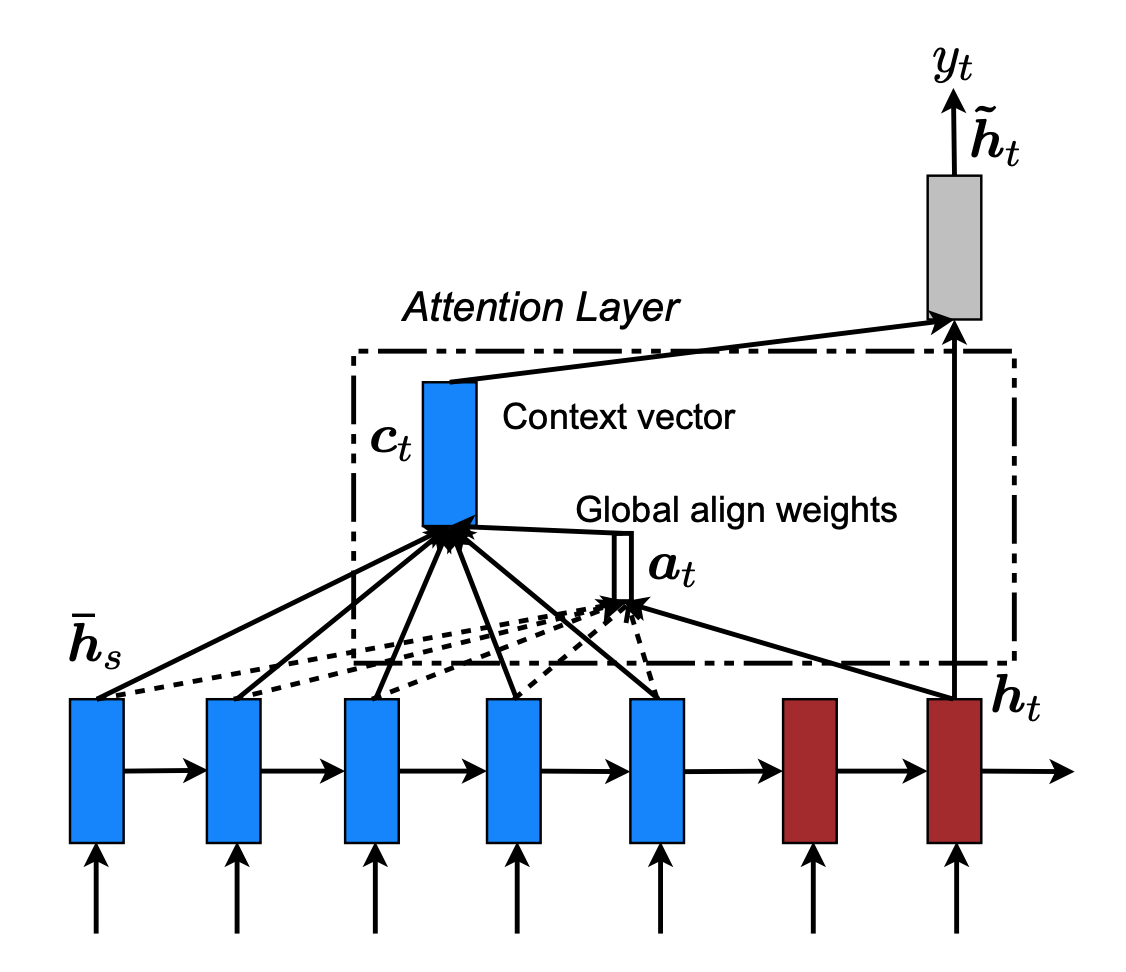
\includegraphics[width=1\textwidth]{fig/globalatn.png}
			\caption{Global Attention Model}
		\end{subfigure}
		\hspace*{\fill} % separation between the subfigures
		\begin{subfigure}{0.3\textwidth}
			\label{fig:localatn}
			\centering
			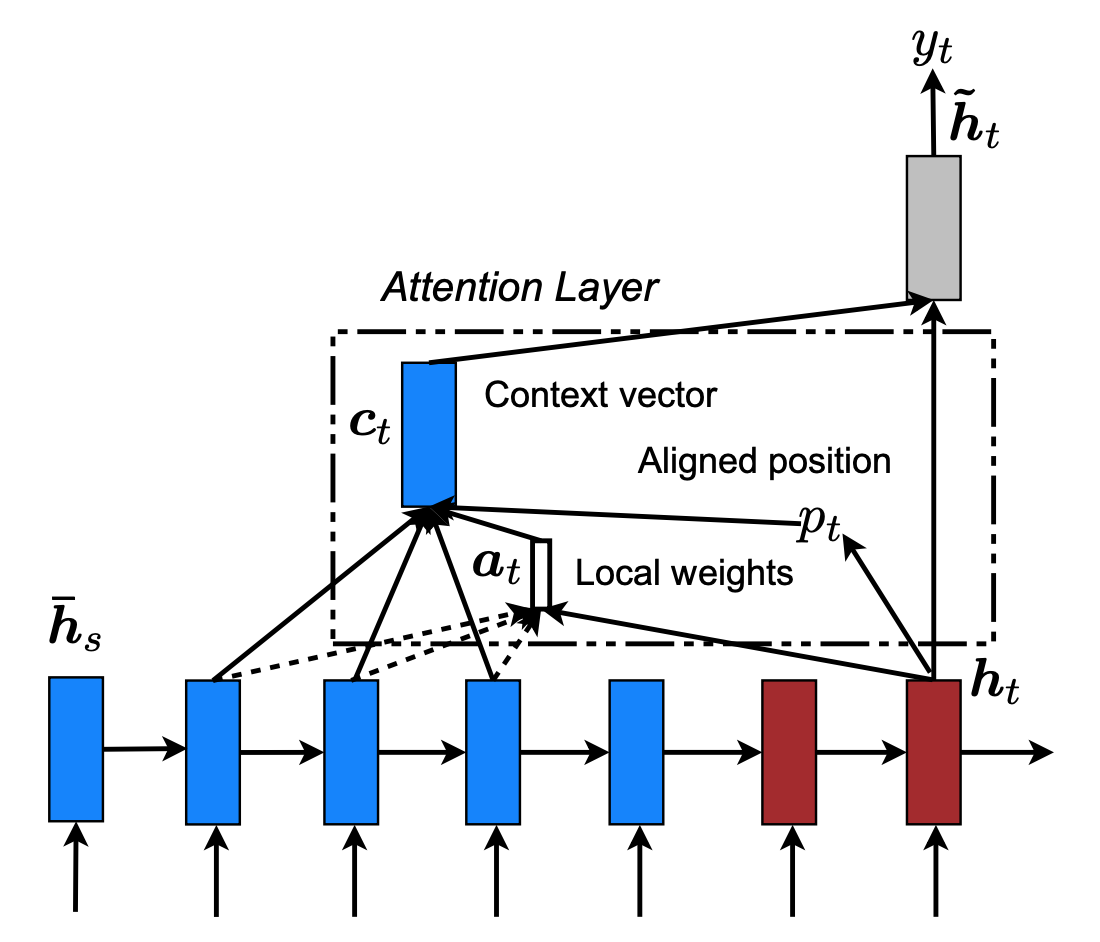
\includegraphics[width=1\textwidth]{fig/localatn.png}
			\caption{Local Attention Model}
		\end{subfigure}
		\hspace{\fill}
		\begin{subfigure}{0.3\textwidth}
			\label{fig:iofeed}
			\centering
			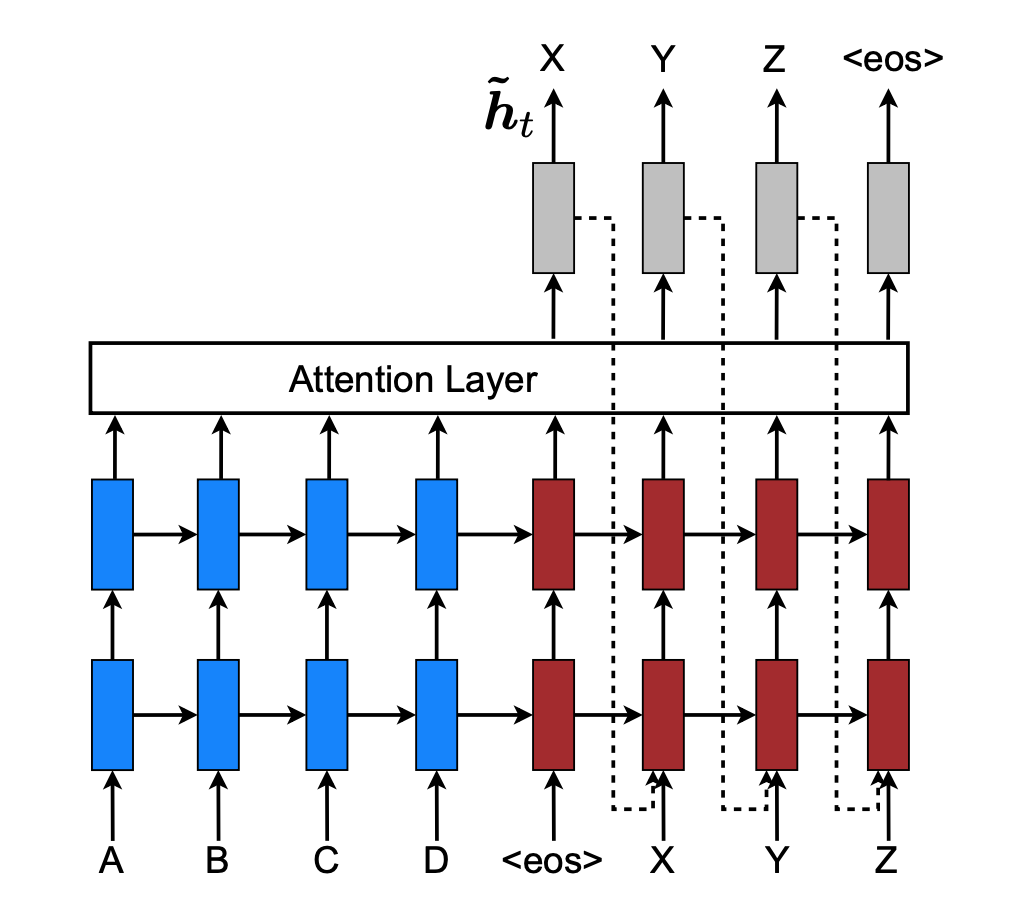
\includegraphics[width=1\textwidth]{fig/iofeed.png}
			\caption{Input-feeeding approach}
		\end{subfigure}
		\caption{The model and the result from Neural Machine Translation by jointly learning to align and translate}
		\label{fig:luong}
	\end{figure}
	
	\paragraph{Global Attention Model: } In this model, a variable length alignment vector \(a_t\) is derived by comparing the current target hidden state \(h_t\) with each source hidden state \(\overline{h_s}\). 
	\[a_t(s) = align(h_t,\overline{h_s}) = \frac{exp(score(h_t, \overline{h_s}))}{\sum_{s'} exp(score(h_t, \overline{h_s'}))}\]
	where the score is referred as a content based function for which the paper provide three alternatives shown in Table \ref{tab:scores}. At each time step \(t\), the model infers a variable-length alignment weight \(a_t\) based on the current target state \(h_t\) and all source states \(\overline{h_s}\). A global context vector \(c_t\) is then created as the weighted average, according to \(a_t\), over all the source states.

	 \begin{table}
	 \caption{Alternatives for \(scores(h_t,\overline{h_s})\)}
	  \centering
	  \begin{tabular}{ll}
	  	\toprule
	    Dot product & \(h_t\overline{h_s}\) \\
	    General     & \(h_t^TW_a\overline{h_s}\) \\
	    Concat     & \(v_a^T\tanh(W_a[h_t;\overline{h_s}])\) \\
	    \bottomrule
	  \end{tabular}
	  \label{tab:scores}
	\end{table}

	\paragraph{Local Attention Model: } This model first predicts a single aligned position \(p_t\) for the current target word at each time step \(t\). As shown in Figure \ref{fig:luong}, a window centered around the source position \(p_t\), \([p_t-D, p_t+D]\) is then used to compute a context vector \(c_t\), a weighted average of the source hidden states in the window. The weights \(a_t\) are inferred from the current target state \(ht\) and those source states \(\overline{h_s}\) in the window. Unlike the global method, the alignment vector is now a fixed dimensional. There were two variants of the model that the authors proposed: 
	\begin{itemize}
		\item \textbf{Monotonic Alignment} (local-m)\\Sets \(p_t = t\) assuming that  and target sequences are roughly monotonically aligned.
		\item \textbf{Predictive alignment} (local-p)\\This model predicts the aligned position as: \(p_t = S \ast sigmoid(v_p^T\tanh(W_ph_t))\). Here \(S\) is the source sentence length. 
	\end{itemize}
	
	\paragraph{Input Feeding Approach: } In standarad MT, to keep track of which source words have been translated, a coverage set is often maintained. To achieve this in NMT, the authors proposed the input-feeeding approach where the attentional vectors \(\widetilde{h_t}\) are fed as inputs to the next time steps to inform the model about past alignment decisions. This has been shown in Figure \ref{fig:luong}.
	
\subsection{Text Understanding with the Attention Sum Reader Network}
\label{sec:kadlec}
	
	Kadlec et al. \cite{kadlec} presented a simple model using attention to directly pick the answer from the context. The raks addressed in this paper consisted of answering a cloze-style question, the answer to which depends on the understanding of a context document. The correct answer was then selected from a set of options. This model was evaluated using CNN and Daily Mail datasets and a Children's Book Test dataset. The core issue that was studied in this paper was that how standard LSTM, which performed at human levels in predicting verbs and prepositions, lagged behind in predicting named entities and common nouns. To test the proposed model the task complexity was varied with the type of word removed. This model assumes that the answer is one of the words in the context.

	\begin{figure}
		\centering
		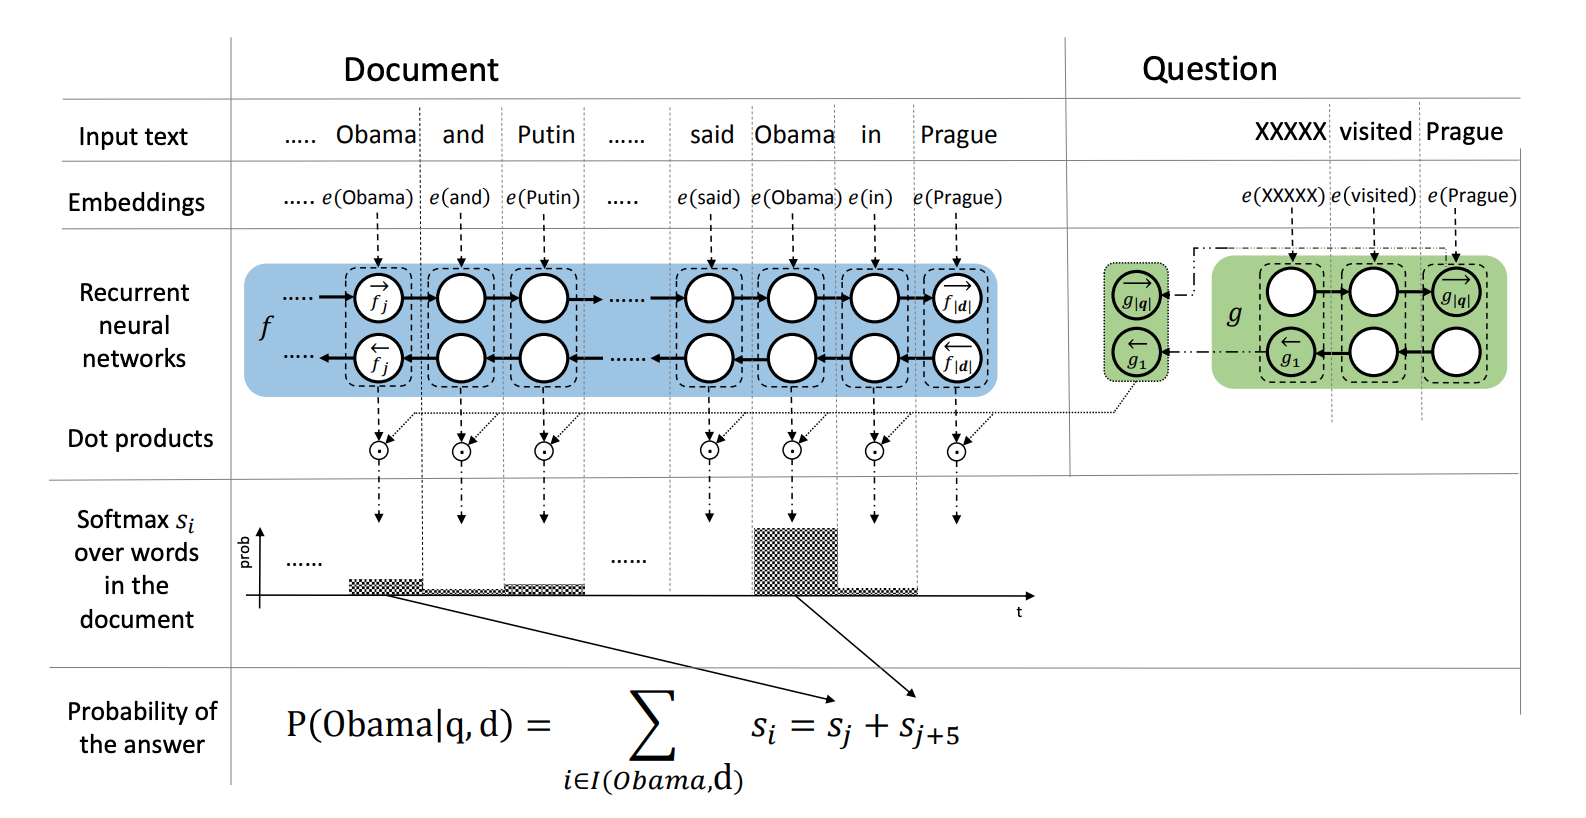
\includegraphics[width=0.9\textwidth]{fig/atnsumrdr.png}
		\caption{The structure of the Attention Sum Reader Network for text understanding.}
		\label{fig:attnsum}
	\end{figure}
	
	\paragraph{Model: } This model comprises two encoder funtion and one embedding function. The word embedding \(e\) translates words into vector representations while the document encoder \(f\) and query  encoder \(g\) encodes the words of context and query \(q\) into \textit{contextual} and \textit{query embeddings} respectively. The contextual embedding of the \(i^{th}\) word in \(d\) is represented as \(f_i(d)\). Now the weight of every word in the document is computed as the dot product of its contextual embedding and the query embedding. The weight here can be viewed as the attention over the document \(d\). The encoders are designed as bidirectional Gated Recurrent Units where the embeddings are concateneted when they interact. The model has been explained in Figure \ref{fig:attnsum}.
	
	One of the major differences of this paper from other attention papers is that it uses a mechanism of pointer sum attention in which it uses attention as a pointer over discrete tokens in the context document and then directly sums the word's attention. On the other hand, in Bahdanau et al. \cite{bahattn}, it used attention to blend representations of words into a new embedding vector. 
	
\subsection{A Structured Self-Attentive Sentence Embedding}
\label{sec:lin}

	In tasks like sentence embedding extraction, people have used attention mechanism on top of CNN or LSTM. However, in cases like sentiment classification where there is only one line given as an input, it is not directly applicable. There have been few approaches like adding a max pooling or averaging step across all time steps, or even just picking up the hidden representation at the lat time step as encode embedding. In this paper by Lin et al. \cite{lin}, they propose a self-attention mechanism for sequential models to replace this max-pooling or averaging step, allowing the model to extract different aspects of the sentence into multiple vector representations. 
	
	\begin{figure}
		\centering
		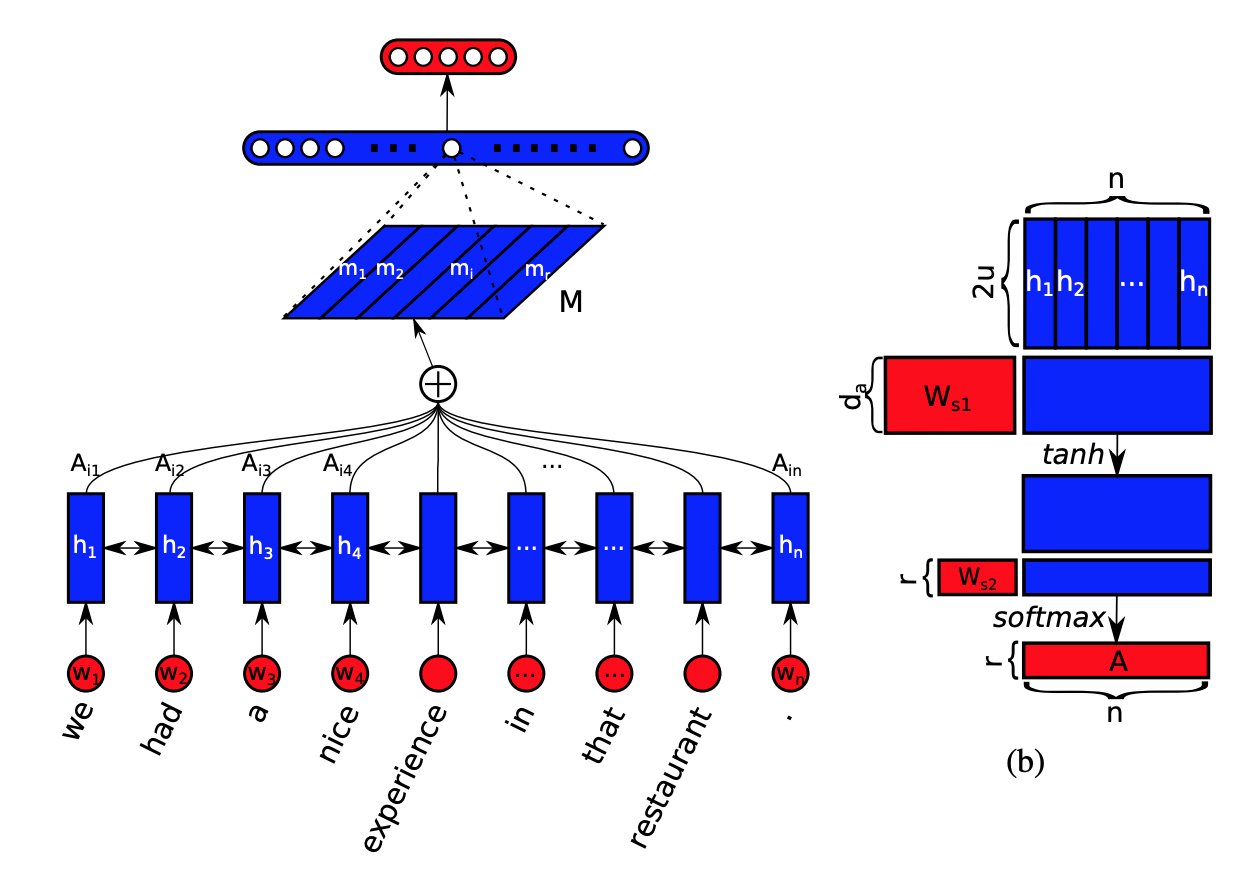
\includegraphics[width=0.75\textwidth]{fig/selfatnemb.png}
		\caption{ A sample model structure showing the sentence embedding model combined with a fully
			connected and softmax layer for sentiment analysis (a). The sentence embedding M is computed as
			multiple weighted sums of hidden states from a bidirectional LSTM \((h_1, ..., h_n)\), where the summation weights \((A_{i_1}, ..., A_{i_n})\) are computed in a way illustrated in (b). Blue colored shapes stand for hidden representations, and red colored shapes stand for weights, annotations, or input/output.}
		\label{fig:attnsum}
	\end{figure}
	
	\paragraph{Model: } Assuming a sentence \(S\) on \(n\) tokens, a Elation Healthdirectional LSTM processes it to produce a concatenated hidden state \(h_t\). In order to encode a variable length sentence into a fixed size embedding, the authors chose a linear combination of the \(n\) LSTM hidden vectors in \(H = (h_1, h_2, ..., h_n)\). Computing this linear combination was done using self-attention mechanism which takes the whole LSTM hidden states \(H\) and ouputs as vector of weights \(a\), where \(s_{s_2}\) is a vector of parameter \(d_a\) which is itself a hyperparameter. 
	\[a = softmax(w_{s_2} \tanh (\textbf{w}_{s_1} H^T))\]
	
	This vector representation focuses on a specific component of a sentence and does not work well when the sentence has multiple aspects and components. Therefore to represent the overall semantics of the sentence, the author's proposed of having multiple \(m\) that would focus on different parts of the sentence. In order to do that, the model has to perform multiple hops of attention so that \(r\) different parts of the sentences are extracted. Hence, they replaced the vector \(w_{s_2}\) with \(W_{s_2}\), a matrix of size \(r \times d_a\).
	\[A = softmax(w_{s_2} \tanh (\textbf{W}_{s_1} H^T))\]
	
	\paragraph{Penalization: } An embedding matrix \(M\) can suffer from redundancy if attention models always provide similat summation weights for all the \(r\) hops. Hence they added a penalization term as 
	\[P = ||AA^T-I||_F^2\]
	
	Here \(||\bullet||\) is the Forbenius norm of a matrix. The authors did not go with KL divergence instead as a penalization term because the vast number of zeros in the annotation matrix \(A\) makes the training unstable. Also KL divergence penalty wouldn't have allowed each individual row to focus on a single aspect of semantics. 
	
\section{Google's Neural Machine Translation System}
\label{sec:goognmt}

	Google's production machine translation system was largely based on phrase-based. NMT, however promissing, were slower in training and inference and were ineffective in dealing with rare words. The paper Wu et al. \cite{goognmt} proposes to solve such problems. The encoders used were LSTM with 8 layers with the first layer being a bidirectional one to gain more context from the input. The decoder is implemented as a combination of RNN network with softmax layer. To model differences between an intermediate layers' outputs, residual connections were used between layers to encourage gradient flow. They also improved the inference time by using low-precision arithmetic for inference computing on special hardware (TPUs). They used attention module similar to Bahdanau et al. \cite{bahattn}. The design has been shown in Figure \ref{fig:goognmt}.
	
	From the rest of the NMT models discussed in previous sections, this paper works forward to gain efficiency in training and inference. The data was processed in parallel by training \(n\) model replicas concurrently which share one copy of model parameters. Each replica updates the parameters asynchronously using a combination of Adam \cite{adam} and SGD algorithms. To achieve model parallelism, the encoder and decoder were partioned along the depth dimension and were placed on multiple GPUs, thus running each layer on each GPU. In the LSTM stack, the layer above bidirectional LSTMs has to wait for both the forward and the backward hidden state computation. Since, this would have caused delays with respect to model parallelism, they used BiLSTM in only the first encoder layer.
	
	One of the biggest problem Machine Translators face is out-of-vocabulary (OOV) words. One common approach is simply copying rare words from source to target based on attention or alignment models. The other one is to use sub-word units like characters, mixed word/characters or more intelligent sub-words. The most successful approach taken in this paper is the Wordpiece model. For processing arbitrary words, the words are first broken into wordpieces using a trained wordpiece model. Given the training corpus and the number of desired tokens \(D\), the optimization problem of this model is to select \(D\) wordpieces such that the resulting corpus is minimal in the number of wordpieces when segmented according to the chosen wordpiece model. A greedy algorithm is used for this purpose \cite{subword}. Sometimes for proper nouns etc it becomes necessary to copy words from source to target sequence. To facilitate this, this model uses a shared wordpiece model for both the source language and target language. This ensures that the same string in the source and the target will be segmented in exactly the same way, making it easier for the system to learn to copy these tokens.
	
	GNMT's quality approached or surpassed all the then published results in machine translation owing to the techniques that were critical to speed, accuracy, robustness. It was able to deal with large datasets and perhaps would have replaced the phrase based MT at Google. The key takeaways from that paper were that wordpiece model effectively handled open vocabularies and that the combination of model and data parallelism can be used to effectively train and infer from the state-of-the-art sequence to sequence NMT models.
	
	\begin{figure}
		\centering
		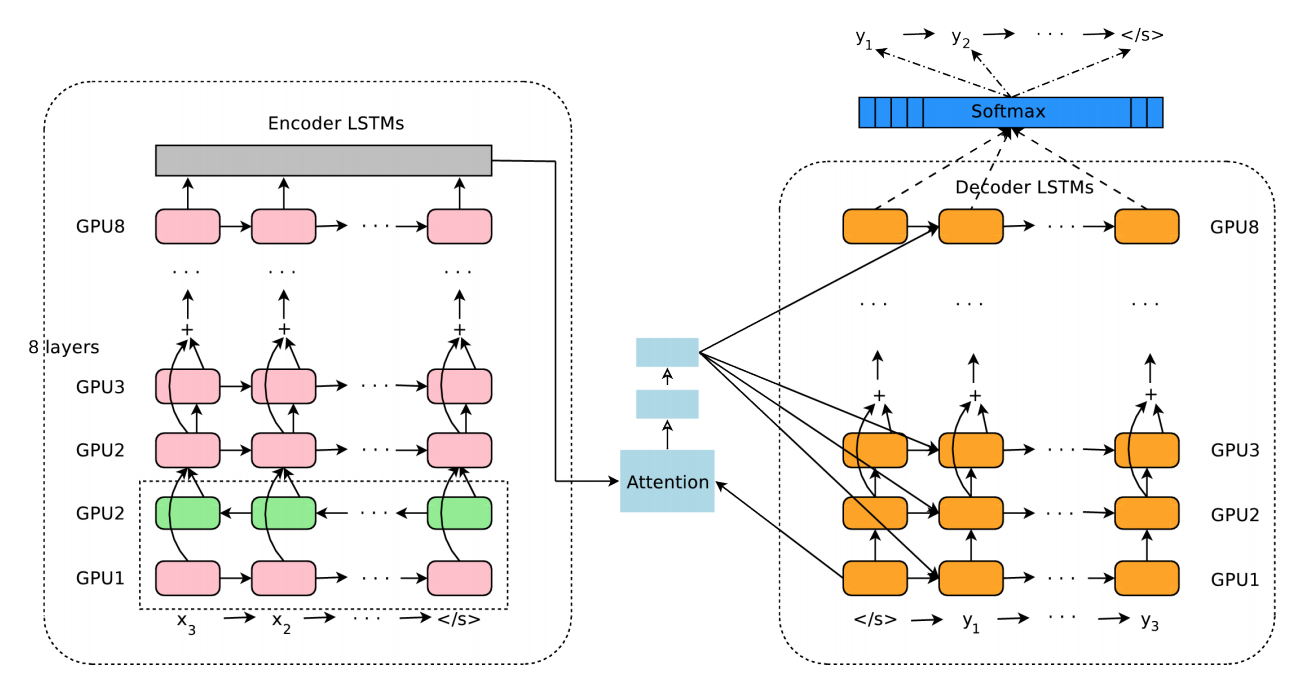
\includegraphics[width=0.95\textwidth]{fig/googatn.png}
		\caption{Google's Neural Machine Translation System. It contains Bi-LSTM in the first layer of encoder. It uses Residual Connections in the encoder and decoder. The model is also partioned into multiple GPUs to speed up training. To retain maximum parallelism, the bottom decoder layer output is used only for obtaining recurrent attention context, which is sent directly ot all the remaing decoder layers. }
		\label{fig:goognmt}
	\end{figure}

\section{Conclusion}
\label{sec:conclusion}
	
	Deep learning offers a way to harness large amount of computation and data with little engineering by hand.  With distributed representation, various deep models have become the new state-of-the-art methods for NLP problems. This survey was focussed on usage of Recurrent Neural Networks architecture and the Attention Mechanism in NLP, specially pertaining to the area of Neural Machine Translation (NMT). We expect more advanced research in this area specifically in attention to make more robust sequence to sequence networks. We put forward a timline in this survey, which started with word representations and how deep learning can better infer from it. We discussed about attention mechanisms like additive, multiplicative and self-attention, that have tremendously improved translation across many NMT models. Even though attention, as presented here, were in line with NLP, we expect it to be used in areas like computer vision, and image analysis, where more relevant information can be extracted using these models. Finally we surveyed Google's GNMT which not only used the state-of-the-art reserach but also made the system production ready. We think of this as a huge step in the direction of Artificial Intelligence. 

\newpage
\bibliographystyle{unsrt}
\bibliography{references}

\newpage
\begin{appendices}
	
\section{Recurrent Neural Network}
\label{sec:rnn}

	RNN is based on the idea of sequential processing. Figure \ref{fig:rnn} introduces the RNN architecture where rectangular box is a hidden layer at a time-step, \(t\). Each such layer holds a number of neurons, each of which performing a linear matrix operation on its inputs followed by a non-linear operation (e.g. \texttt{tanh()}). At each time-step, the output of the previous step along with the next word vector in the document, \(x_t\), are inputs to the hidden layer to produce a prediction output \(\hat{y}\) and output features \(h_t\). 
	\[
		h_t = \sigma(W_{hh}h_{t-1} + W_{hx}x_{[t]}) \label{eq:1} \tag{1}  
	\]
	\[
		\hat{y_t} = softmax(W^{(S)} h_t) \label{eq:2} \tag{2}
	\]
	
	Here, \((x_1,... x_T)\) are the word vectors corresponding to a corpus with \(T\) words. \(W^{hh} \in \Re^{D_h \times D_h} \) is the weights matrix used to condition the output of the previous time-step, \(h_{t-1}\). \(W^{hx} \in \Re^{D_h \times d} \) is the weights matrix used to condition the input word
	vector, \(x_t\). 
	
	The loss function used in RNNs is often the cross entropy error. The cross entropy error over a corpus of size \(T\) summed over all the vocabulary words is:
	\[J = -\frac{1}{T} \sum_{t=1}^{T} \sum_{j=1}^{|V|} y_{t,j} \times log(\hat{y_{t,j}}) \tag{3}\]
	
	The amount of memory required to run a layer of RNN is proportional to the number of words in the corpus. For instance, a sentence with \(k\) words would have \(k\) word vectors to be stored in memory. Also, the RNN must maintain two pairs of \(W\), \(b\) matrices. While the size of \(W\) could be very large, it does not scale with the size of the corpus.
	
	\begin{figure} [H]
		\centering
		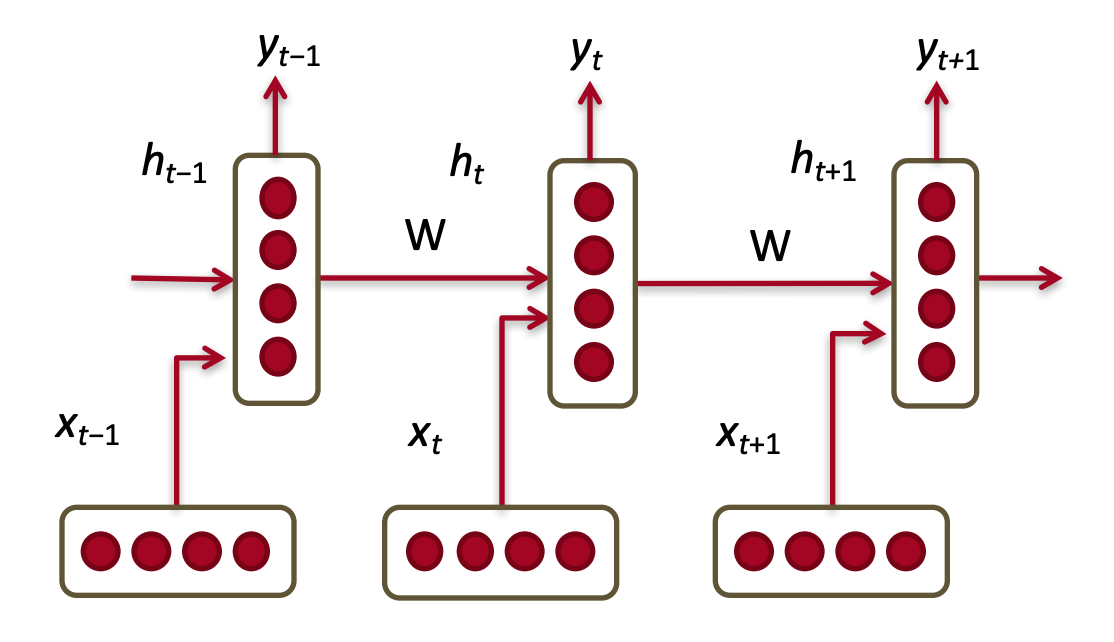
\includegraphics[width=0.3\textwidth]{fig/rnn.png}
		\caption{A Recurrent Neural Network Unit}
		\label{fig:rnn}
	\end{figure}
	
\section{Vanishing Gradients and Explosion Problems}
\label{sec:van}

	Consiter at a time step \(t\), to compute RNN error gradient, \(dE/dW\), we sum the error at each time-step ie. \(dE_t/dW\) is computed for every time-step \(t\), and accumulated.
	\[\frac{\partial E}{\partial W} = \sum_{t=1}^{T} \frac{\partial E_t}{\partial W} \tag{4}\]
	
	The error for each time-step is computed through applying the chain rule differentiation to Equations (1) and (2); Equation 5 shows the differentiation. Note that \(dh_t/dh_k\) refers to the partial derivative of \(h_t\) with respect to all previous \(k\) time-steps.
	
	\[
		\frac{\partial E_t}{\partial W} = \sum_{k=1}^{t} \frac{\partial E_t}{\partial y_t} \frac{\partial y_t}{\partial h_t} \frac{\partial h_t}{\partial h_k} \frac{\partial h_k}{\partial W}
		\tag{5}
	\]
	
	Equation 6 shows the relationship to compute each \(dh_t/dh_k\); this is simply a chain rule differentiation over all hidden layers within the \([k, t]\) time interval.
	
	\[
		\frac{\partial h_t}{\partial h_k} = \prod_{j=k+1}^{t} \frac{\partial h_j}{\partial h_{j-1}} = \prod_{j=k+1}^{t} W^T \times diag(f'(j_{j-1}))
		\tag{6}
	\]
	
	Since \(h \in \Re^{D_n} \), each \(\partial h_j/\partial h_{j-1} \) is the Jacobian matrix for \(h\). Putting Equations 4,5,6 together we have:
	\[
		\frac{\partial E}{\partial W} = \sum_{t=1}^{T} \sum_{k=1}^{t} \frac{\partial E_t}{\partial y_t} \frac{\partial y_t}{\partial h_t} (\prod_{j=k+1}^{t} \frac{\partial h_j}{\partial h_{j-1}}) \frac{\partial h_k}{\partial W}
		\tag{7}
	\]
	
	Equation 8 shows the norm of the Jacobian matrix relationship. Here, \(\beta_W\) and \(\beta_h\) represent the upper bound values for the two matrix norms. The norm of the partial gradient at each time-step, \(t\), is therefore, calculated through the relationship shown in Equation 8.
	\[
		\parallel \frac{\partial h_j}{\partial h_{j-1}} \parallel \leq \parallel W^T \parallel \parallel diag(f'(j_{j-1})) \parallel \leq \beta_W \beta_h
		\tag{8}
	\]
	
	The norm of both matrices is calculated through taking their L2-norm. The norm of \(f'(j_{j-1})\) can only be as large as 1 given the sigmoid non-linearity function.
	
	\[
		\parallel \frac{\partial h_t}{\partial h_k} \parallel = \parallel \prod_{j=k+1}^{t} \frac{\partial h_j}{\partial h_{j-1}} \parallel \leq (\beta_W \beta_h)^{t-k}
		\tag{9}
	\]
	
	The exponential term \((\beta_W \beta_h)^{t-k}\)  can easily become a very small or large number when \(\beta_W \beta_h\) is much smaller or larger than \(1\) and \(t-k\) is sufficiently large. In case of language models, the contribution of faraway words to predicting the next word at time-step \(t\) diminishes when the gradient vanishes early on.
	
	During experimentation, once the gradient value grows extremely large, it causes an overflow which is easily detectable at runtime; this issue is called the Gradient Explosion Problem. When the gradient value goes to zero, however, it can go undetected while drastically reducing the learning quality of the model for far-away words in the corpus; this issue is called the Vanishing Gradient Problem.
	
\section{Gated Recurrent Units}
\label{sec:gru}

	Although RNNs can theoretically capture long-term dependencies, they are very hard to actually train to do this. Gated recurrent units are designed in a manner to have more persistent memory thereby making it easier for RNNs to capture long-term dependencies. The architecture is defined as:
	\[
	z_t = \sigma (W^{(z)}x_t + U^{(z)}h_{t-1}) \tag{Update Gate}
	\]
	\[
	r_t = \sigma (W^{(r)}x_t + U^{(r)}h_{t-1}) \tag{Reset Gate}
	\]
	\[
	\widetilde{h_t} = \tanh (r_t \circ Uh_{t-1} + Wx_t) \tag{New Memory}
	\]
	\[
	h_t = (1-z_t) \circ \widetilde{h_t} + z_t \circ h_{t-1} \tag{Hidden State}
	\]
	
	The above equations can be thought of a GRU’s four fundamental operational stages:
	\begin{enumerate}
		
		\item \textbf{New memory generation:} A new memory  \(\widetilde{h_t}\) is the consolidation of a new input word \(x_t\) with the past hidden state \(h_{t-1}\). Anthropomorphically, this stage is the one who knows the recipe of combining a newly observed word with the past hidden state \(h_{t-1}\) to summarize this new word in light of the contextual past as the vector \(\widetilde{h_t}\).
		
		\item \textbf{Reset Gate:} The reset signal \(r_t\) is responsible for determining how important \(h_{t-1}\) is to the summarization \(\widetilde{h_t}\). The reset gate has the ability to completely diminish past hidden state if it finds that \(h_{t-1}\) is irrelevant to the computation of the new memory.
		
		\item \textbf{Update Gate:} The update signal \(z_t\) is responsible for determining how much of \(h_{t-1}\) should be carried forward to the next state. For instance, if \(z_t \approx 1\), then \(h_{t-1}\) is almost entirely copied out to \(h_t\). Conversely, if \(z_t \approx 0\), then mostly the new memory \(\widetilde{h_t}\) is forwarded to the next hidden state.
		
		\item \textbf{Hidden state:} The hidden state \(h_t\) is finally generated using the past hidden input \(h_{t-1}\) and the new memory generated \(\widetilde{h_t}\) with the advice of the update gate.
		
	\end{enumerate}

\section{Long Short Term Memory}
\label{sec:lstm}

	Long-Short-Term-Memories are another type of complex activation unit that differ a little from GRUs. The motivation for using these is similar to those for GRUs however the architecture of such units does differ.
	\[
	i_t = \sigma (W^{(i)}x_t + U^{(i)}h_{t-1}) \tag{Input Gate}
	\]
	\[
	f_t = \sigma (W^{(f)}x_t + U^{(f)}h_{t-1}) \tag{Forget Gate}
	\]
	\[
	o_t = \sigma (W^{(o)}x_t + U^{(o)}h_{t-1}) \tag{Output Gate}
	\]
	\[
	\widetilde{c_t} = \tanh (W^{(c)}x_t + U^{(c)}h_{t-1}) \tag{New Memory Cell}
	\]
	\[
	c_t = i_t \circ \widetilde{c_t} + f_t \circ c_{t-1} \tag{Final Memory Cell}
	\]
	\[
	h_t = o_t \circ \tanh (c_t)
	\]
	
	The above equations can be explained as:
	
	\begin{enumerate}
		
		\item \textbf{New memory generation:} Analogous to GRU.
		 		
		\item \textbf{Input Gate:} The new memory generation stage doesn’t check if the new word is even important before generating the new memory – this is exactly the input gate’s function. The input gate uses the input word and the past hidden state to determine whether or not the input is worth preserving and thus is used to gate the new memory. It thus produces \(i_t\) as an indicator of this information.
		
		\item \textbf{Forget Gate:} This gate is similar to the input gate except that it does not make a determination of usefulness of the input word – instead it makes an assessment on whether the past memory cell is useful for the computation of the current memory cell. Thus, the forget gate looks at the input word and the past hidden state and produces \(f_t\).
		
		\item \textbf{Final memory generation:} This stage first takes the advice of the forget gate \(f_t\) and accordingly forgets the past memory \(c_{t-1}\). Similarly, it takes the advice of the input gate \(i_t\) and accordingly gates the new memory \(\widetilde{c_t}\). It then sums these two results to produce the final memory \(c_t\).
		
		\item \textbf{Output/Exposure Gate:} This is a gate that does not explicitly exist in GRUs. It’s purpose is to separate the final memory from the hidden state. The final memory \(c_t\) contains a lot of information that is not necessarily required to be saved in the hidden state. Hidden states are used in every single gate of an LSTM and thus, this gate makes the assessment regarding what parts of the memory \(c_t\) needs to be exposed/present in the hidden state \(h_t\). The signal it produces to indicate this is \(o_t\) and this is used to gate the point-wise \(\tanh\) of the memory.
		
	\end{enumerate}

	\begin{figure}
		\centering
		\begin{subfigure}{0.4\textwidth}
			\label{fig:gru}
			\centering
			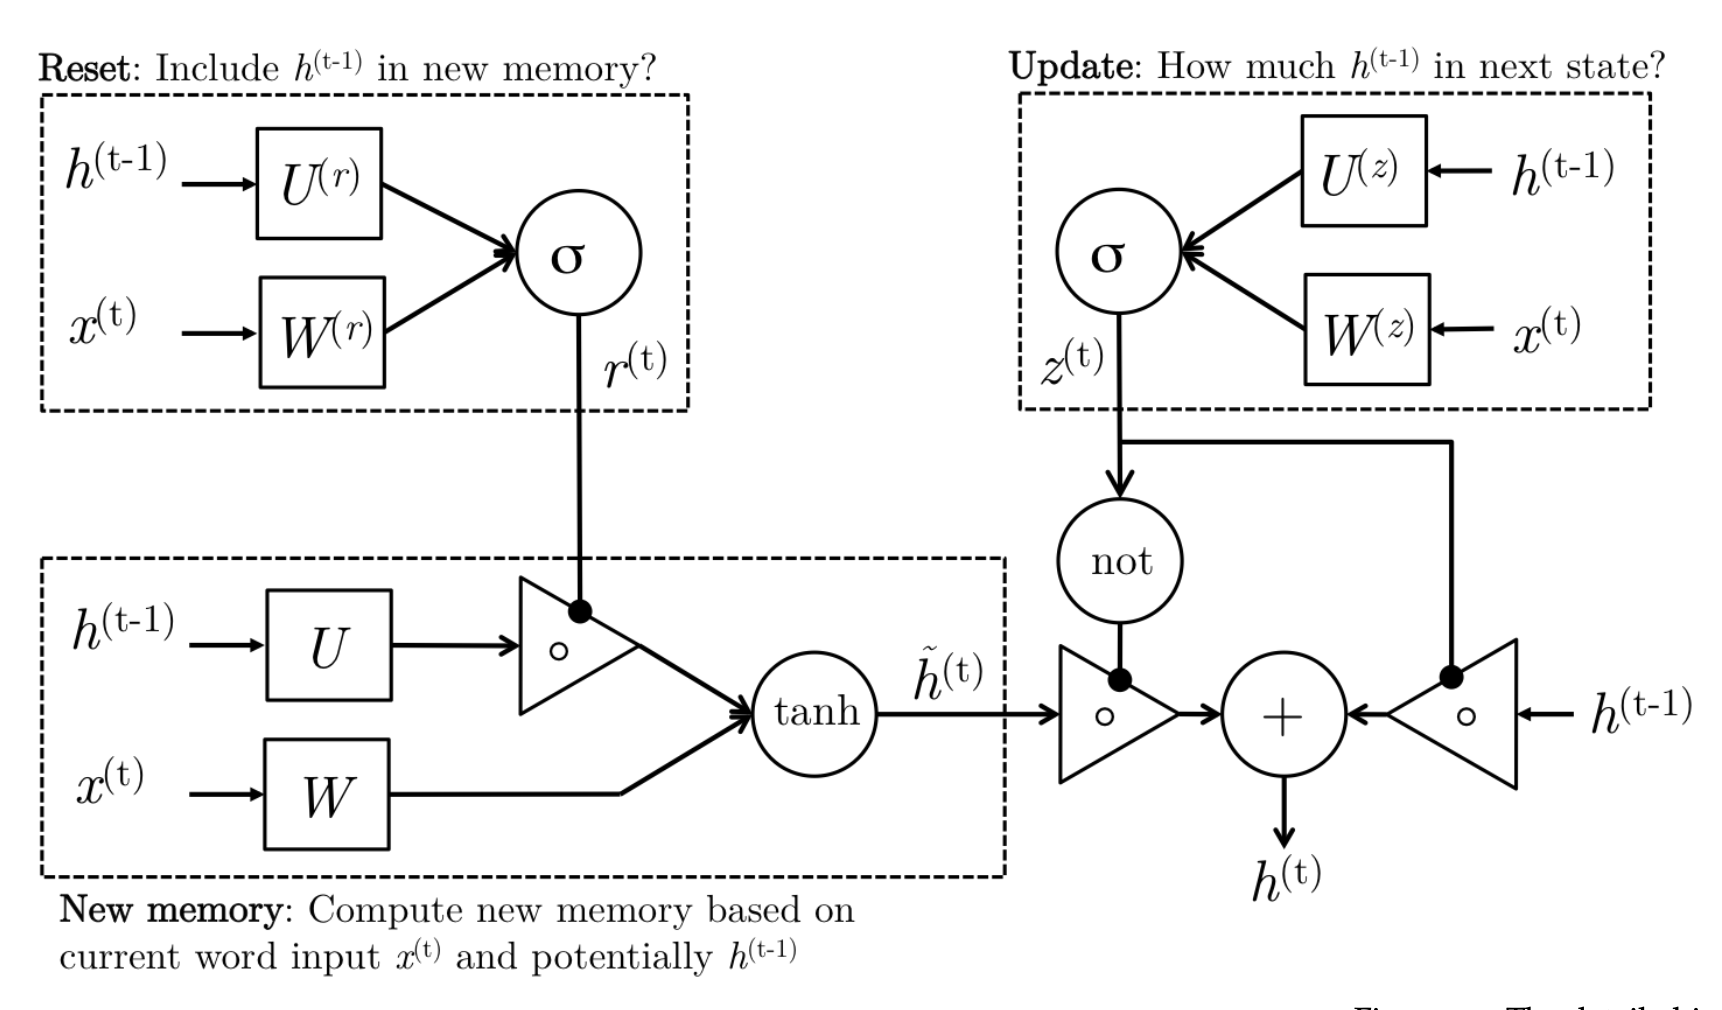
\includegraphics[width=1\textwidth]{fig/gru.png}
			\caption{Gated Recurrent Unit}
		\end{subfigure}
		\hspace*{\fill} % separation between the subfigures
		\begin{subfigure}{0.4\textwidth}
			\label{fig:lstm}
			\centering
			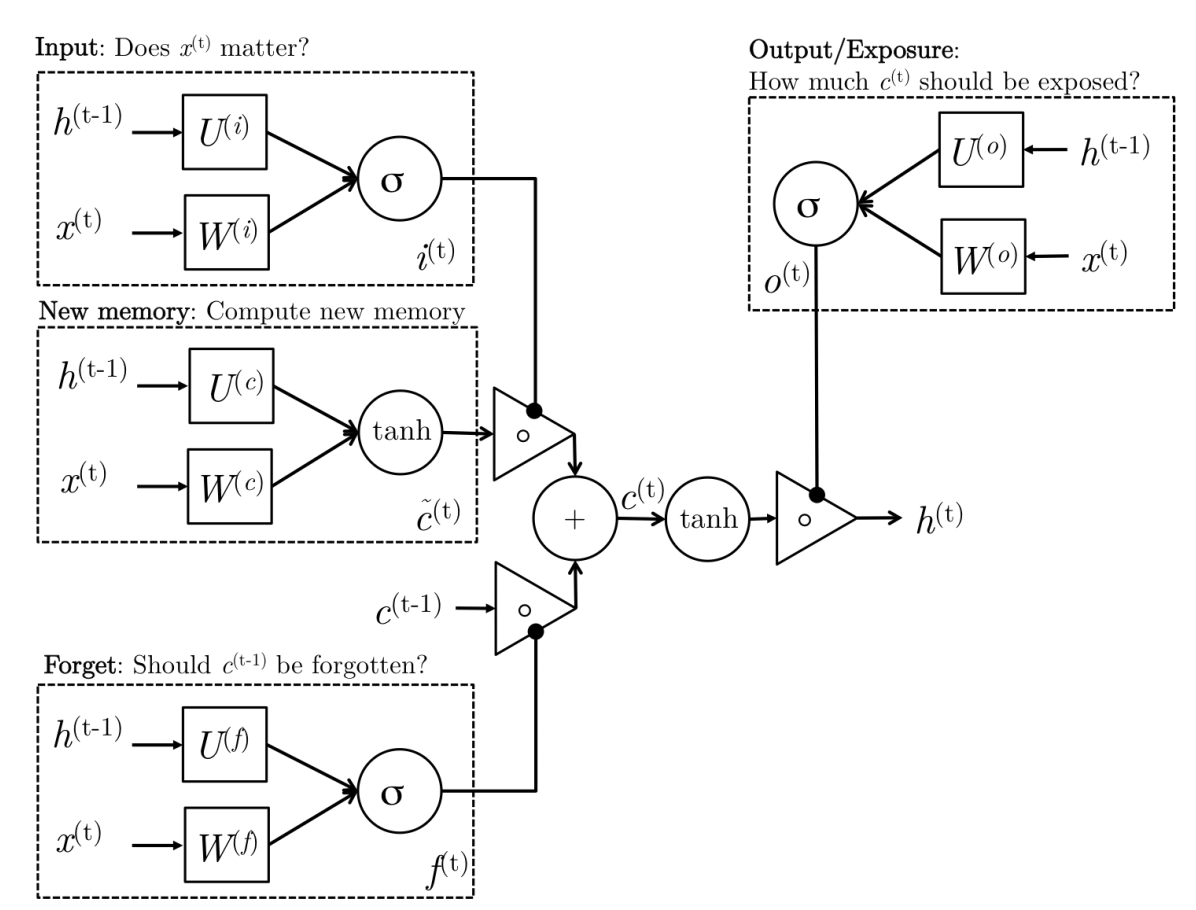
\includegraphics[width=1\textwidth]{fig/lstm.png}
			\caption{Long Short Term Memory Unit}
		\end{subfigure}
		\caption{Variants of RNN}
		\label{fig:rnna}
	\end{figure}

\end{appendices}

\end{document}

